\documentclass[a4paper,journal]{IEEEtran}

\usepackage{cite}
% \usepackage[nocompress]{cite}
\usepackage{ifpdf}

\ifpdf
\usepackage[pdftex]{graphicx}
\graphicspath{{./img/}}
\DeclareGraphicsExtensions{.pdf}
\else
\usepackage[dvips]{graphicx}
\graphicspath{{./img/}}
\DeclareGraphicsExtensions{.eps}
\fi

\usepackage[cmex10]{amsmath}
\usepackage{amsfonts}
\usepackage{amssymb}
\interdisplaylinepenalty=2500

\usepackage[margin=15mm]{geometry}

\usepackage{algorithmic}

\usepackage{array}

\usepackage{mdwmath}
\usepackage{mdwtab}

\usepackage{eqparbox}

\usepackage[hang,small,center,bf]{caption}
% \usepackage[tight,normalsize,sf,SF]{subfigure}
%\usepackage[tight,footnotesize]{subfigure}
\usepackage{subfig}
% \usepackage[caption=false,font=normalsize,labelfont=sf,textfont=sf]{subfig}
% \usepackage[caption=false,font=footnotesize]{subfig}

\usepackage[utf8x]{inputenc}
\usepackage[czech]{babel}
\usepackage[colorlinks=true,urlcolor=blue]{hyperref}
\usepackage{url}
\usepackage{fixltx2e}
\usepackage{stfloats}
\usepackage{ucs}
\usepackage{multirow}

% correct bad hyphenation here
\hyphenation{op-tical net-works semi-conduc-tor}

\renewcommand{\labelitemi}{$\bullet$}
\renewcommand{\labelitemii}{$\circ$}
\renewcommand{\labelitemiii}{$\ast$}

\setlength{\textheight}{260mm}

\begin{document}

\title{Návrh a verifikace řídícího systému pro nádraží}
\date{August 8, 2012}
\author{Peter~Boráros%
%\thanks{{Peter Boráros}, CTU FEE,
%see~\url{http://www.pborky.sk/contact} for a contact infomation}%
}%

% The paper headers
%\markboth{Peter Boráros, Czech technical university, Faculty of Electrical Engineering, Prague, Czech Republic}{}

\IEEEcompsoctitleabstractindextext{%
\begin{abstract}
Tento dokument popisuje řešení semestrální úlohy pro kurz a4m33au - automatické uvažování.
Cílem je návrh a verifikace řídícího systému pro vlakové nádraží, s použitím automatického
dokazování v logice prvního řádu.
\end{abstract}}

\maketitle
\IEEEdisplaynotcompsoctitleabstractindextext
\IEEEpeerreviewmaketitle

\section{Úvod}\label{sec:intro}
Táto práce představuje návrh a verifikaci řídícího systému pro vlakové nádraží, s použitím automatického
dokazování v logice prvního řádu.

V sekci \ref{sec:intro} je popsané podrobné zadání problému (je převzaté z webových stránek kurzu). 
V sekci \ref{sec:formal} přecházi přes jednotlivé aspekty problému, formalizuje je a přináší obecné řešení. 
Sekce \ref{sec:imple} popisuje implementaci a způsob použití navrženého systému. V sekci 
\ref{sec:exp} je rozbor experimentů, nad jednoduchými instancemi problému (vid obr. 
\ref{fig:nad1}, \ref{fig:nad2} a \ref{fig:nad3}),
a závěr.

\subsection{Specifikace problému}
Nádraží je souvislý orientovaný graf. Uzly, z kterých nevedou šipky, nazveme výjezdy, uzly, 
do kterých nevedou vedou šipky, nazveme vjezdy. Omezujeme se na grafy, u kterých 
z každého vjezdu existuje cesta do každého výjezdu. Každý uzel a každá hrana mají 
zadaný unikátní název (začínající malým písmenem).

\subsubsection{Vlastnosti nádraží}
\begin{itemize}
	\item Každý uzel s více než jednou výstupní hranou je zároveň výhybka.
	\item Časově variabilní prvky v nádraží jsou:
	\begin{itemize}
		\item pohybující se vlaky,
		\item na vstupních uzlech řízená návěstidla a
		\item výhybky.
	\end{itemize}
	\item V daném časovém okamžiku je každý vlak právě v jednom uzlu.
	\item Vlaky se pohybují pouze ve směru orientace hran grafu (tj. nemohou couvat).
	\item Je-li v uzlu vlak, platí, že vlak někdy do uzlu přijel (nebyl tam od nepaměti) 
	a jednou odjede (ale není určeno, kdy - je to na ,,rozhodnutí strojvedoucího``).
	\item Na vjezdových uzlech (a pouze tam) jsou návěstidla. Ta blokují odjezd vlaků 
	ze vstupních uzlů: Je-li návěstidlo zavřené, vlak zůstává na vstupním uzlu; 
	je-li otevřené, může (ale nemusí) vyjet. Vlak (strojvedoucí) vždy tato návěstidla 
	respektuje. Každý vjezdový uzel má právě jednu výstupní hranu, není tedy nikdy výhybkou.
	\item Každý vlak má dán výstupní uzel, do kterého chce dojet. Tento cíl se nemění 
	celou dobu, co vlak projíždí nádražím.
	\item Nádraží podle tohoto cíle směruje vlak pomocí přepínání výhybek. 
	Řídící systém nádraží může libovolně nastavovat stav výhybek.
	\item Pokud je vjezdový uzel prázdný, může se v něm kdykoliv objevit nový 
	přijíždějící vlak (i hned po odjezdu předcházejícího).
\end{itemize}

\subsubsection{Kritické stavy v nádraží}
V nádraží rozlišujeme tyto kritické stavy:
\begin{itemize}
	\item Vlak stojí v uzlu (který je zároveň výhybkou, viz výše), a dojde k přepnutí výhybky.
	\item Dva nebo více vlaků přijede do stejného uzlu.
	\item Vstupní návěstidlo zůstane trvale uzavřené.
\end{itemize}

\subsubsection{Vstup}
Graf nádraží bude zadáván v následujícím formátu 
(podmnožina jazyka DOT \cite{Graphviz}):

\begin{verbatim}
digraph nadrazi_1 { 
  vjezd1 -> uzel1; 
  ...
  uzel1 -> vyjezd1; 
  uzel1 -> vyjezd2; 
} 
\end{verbatim}

\subsubsection{Výstup}
Úkolem je navrhnout program, který
\begin{itemize}
	\item pro zadané nádraží navrhne řídící systém a zformalizuje podle uvedeného zadání;
	\item dokáže, že navržený řídící systém pracuje správně, tj. že se nádraží nemůže dostat 
	do kritického stavu.
\end{itemize}

\subsubsection{Automatické dokazování}
Nádraží je modelováno v diskrétním čase. Čas je lineární, a každý časový okamžik má právě jeden následující a jeden předcházející. V každý časový okamžik si řídící systém nádraží určuje stavy výhybek a návěstidel.

Úkoly, které postupně zpracuje program pro libovolné nádraží pomocí nástrojů pro automatické dokazování:

\begin{itemize}
	\item Formalizace nádraží:
	\begin{itemize}
		\item Zformalizovat v logice 1. řádu v jazyce TPTP ,,fyzikální chování`` nádraží, 
		tedy jak vlaky projíždějí nádražím na základě návěstidel a ,,rozhodování strojvedoucích``. 
		Každý predikát p závislý na čase popisující něco, co dovedeme určit, musí být popsaný nejvýše 
		jednou formulí tvaru $p(T+1) \Leftrightarrow \phi$, kde $\phi$ je formule závislá pouze 
		na okolnostech v čase $T$ a dřívějších (tím je syntakticky zaručena korektnost definice).
		Do toho spadá zejména stav výhybek, zda je v daném uzlu vlak, atd. 
		Nespadá sem především vůle strojvedoucího, kterou neznáme
		(jen víme, že vždy nakonec s vlakem odjede).
		\item Ukázat, že tato formalizace není sporná s přidanými podmínkami, že strojvůdce vlaku jede hned,
		jakmile může, a že do nádraží vjede vlak vždy, jakmile může.
	\end{itemize}
	\item Zformalizovat návrh řídícího systému stejným způsobem jako v predešlém bodě.
	\item Ukázat, že je výsledná formalizace nádraží a jeho řízení bezesporná.
	\item Dokázat, že nikdy nenastane kritický stav.
	\item Nádraží musí pouštět vlaky hned, jakmile je to možné. 
	Je třeba dokázat pro nejaké nádraží s jedním vstupem, že budou-li v čase $t$ v tomto nádraží 2 vlaky, 
	jeden nebo víc vlaků na výstupu a jeden na vstupu, že se návěstidlo na vstupu v čase $t+1$ otevře.
\end{itemize}


\section{Formalizace problému}\label{sec:formal}
\subsection{Reprezentace grafu v logice prvního řádu}
Vlakové nádraží je popsané orientovaným grafem. V níže popsané logické struktuře vrcholy grafu
představují konstantné symboly (napr. vrchol $a$ je popsaný symbolem $a/0$).
Orientované hrany jsou popsane binárním predikátem $edge/2$. Term $edge(a,b)$ říká, že v grafu je přítomna 
hrana $\langle a,b\rangle$ a naopak neprítomnost této hrany je určena termem $\neg edge(a,b)$.
Pro úplný popis grafu je potrebné specifikovat, které hrany jsou přítomny, a které přítomny nejsou,
t.j.:
\begin{equation}
( \bigwedge_{\langle a,b\rangle\in G}{edge(a,b)} ) \wedge 
( \bigwedge_{\langle a,b\rangle\not\in G}{\neg edge(a,b)} )\;.
\end{equation}

Dále nasleduje definice orientované cesty v grafu, reprezentované predikátem $path/2$. Hrana je zároven (elementární) cesta:
\begin{equation}
\forall a,b: edge(a,b) \Rightarrow path(a,b)\;,
\end{equation}
a dále, cesta je tranzitivní:
\begin{equation}
	\forall a,b,c: path(a,b)\wedge path(b,c) \Rightarrow path(a,c)\;.
	%\footnote[1]{z důvodu lepší citelnosti jsou opomenuty závorky a budeme spoléhat na pravidla asociativity }
\end{equation}


Jestě je potřeba popsát vstupní, výstupní a divergetní uzly.
Predikát $input/1$ je definován:
\begin{equation}
\forall x: input(x) \Leftrightarrow \bigvee_{y \in in(G)} (x=y)\;,
\end{equation}
kde funkce $in$ vrací množinu uzlů, do kterých nevede žádná hrana. Dále predikát $output/1$:
\begin{equation}
\forall x: output(x) \Leftrightarrow \bigvee_{y \in out(G)} (x=y)\;,
\end{equation}
kde funkce $out$ vrací množinu uzlů, ze kterých nevede žádná hrana. A koněčne predikát $diverge/1$:
\begin{equation}
\forall x: diverge(x) \Leftrightarrow \bigvee_{y \in more(G)} (x=y)\;,
\end{equation}
kde funkce $more$ vrací množinu uzlů, s více než jedním potomkem.


\subsection{Definice diskrétního času}
Nejprve je potřebné definovat predikát lineárního uspořádaní $less$. 
Ten je definovaný následujícímy axiomy:
\begin{equation}\label{eq:ltlantisym}
\forall x,y:  less(x,y) \wedge less(y,x)\Rightarrow (x = y)
\end{equation}
\begin{equation}\label{eq:ltltran}
\forall x,y,z: less(x,y) \wedge less(y,z) \Rightarrow less(x,z) 
\end{equation}
\begin{equation}\label{eq:ltltotal}
\forall x,y: less(x,y) \vee less(y,x)
\end{equation}
Vztahy (\ref{eq:ltlantisym}), (\ref{eq:ltltran}) a (\ref{eq:ltltotal}) představují antisymetrii,
tranzitivitu a úplnost lineárního uspořádání.

S pomocí výše uvedeného predikátu $less/2$ definujeme funkci $succ/1$, která představuje přímeho následníka:
\begin{equation}
\begin{split}
\forall x:less(x,succ(x)) \wedge
(\forall y:less(y,x) \vee 
less(succ(x),y))
\end{split}
\end{equation}
a dále musí platit:
\begin{equation}\label{eq:succ_neq}
\forall x: succ(x) \not = x
\end{equation}

Funkci $succ$ je možné použít k vyjádření následujícího časového okamžiku.
Napr. hodnota $succ(succ(T))$ představuje posunutí o dva okamžiky vpřed proti hodnote $T$.

\subsection{Pohyb vlaku}
Poloha a smeřování vlaku v čase jsou určeny predikátem $at/3$; term $at(t,y,u)$ říká, že v čase $t$, v uzlu $y$ je vlak směřující do
uzlu $u$. Víme, že vlak směřující do uzlu $u$ je v nejakém uzlu $y$ v nejakém čase $succ(t)$ tehdy a jen tehdy, byl-li v daném uzlu
v předešlém okamžiku a ,,nechtěl`` nebo nemohl z neho vyjet, anebo byl v předešlém uzlu a mohl a zároveň ,,chtěl`` vyjet:
\begin{equation}\label{eq:move}
\begin{split}
\forall t,y,u:&\; at(succ(t),y,u) \Leftrightarrow\\
&(at(t,y,u) \wedge \neg (want(t,y) \wedge \exists z:may(t,y,z))) \vee\\
&(at(t,x,u) \wedge want(t,x) \wedge may(t,x,y))\\ 
\end{split}
\end{equation}
Predikát $want/2$ představuje ,,vůli`` strojvůdce, t.j. $want(t,x)$ znamená, že v čase $t$ se ,,chce`` posunout z uzlu $x$ dále.
Predikát $may/3$ představuje možnost pokračovat, t.j. je-li u vstupů otevřené návěstidlo, případne u divergentního spojení sepnuta výhybka v daném směru, u ostatních uzlú možnosť pokračovat není omezena - 
vlak může vyjet jakmile strojvůdce ,,chce``.
Term $may(t,x,y)$ znamená, že vlak může v čase $t$ postoupit z uzlu $x$, do uzlu $y$. 
\begin{equation}
\begin{split}
\forall t,y,u: may(t,x,y) \Leftrightarrow &\; edge(x,y) \wedge \\
( (input(x) \wedge &\; signal(t,x) ) \vee \\
(diverge(x) \wedge &\; branch(t,x,y)) \vee \\
(\neg diverge(x) \wedge &\; \neg input(x) ))
\end{split}
\end{equation}

Dle zadání víme, že vlak do uzlu jednou přišel a taky, že jednou odjede. ,,Vůli`` strojvůdce je tedy možno definovat
vzhledem k výskytu vlaku v nejakém uzlu:
\begin{equation}
\begin{split}
	\forall t,x,u: &\;(at(t,x,u) \wedge input(x) \wedge signal(t,x)) \Rightarrow \\
	\Rightarrow &\; want(t,x)\\
\end{split}
\end{equation}
\begin{equation}
\begin{split}
\forall t,x,u: &\;((at(t,x,u) \wedge \neg input(x)) \Rightarrow \\
\Rightarrow&\;(\exists t_1: less(t,t_1) \wedge want(t_1,x) ) \;,\\
\end{split}
\end{equation}
t.j. pokud je vlak na vstupu a může vyjet, tak tak strojvůdce ,,chce`` vyjet, když na vstupu není 
tak bude chtít pokračovat v nejaký následujíci okamžik.

Je ale taky nutné ověřit jestli je formalizace není sporná, 
když přidáme podmínku, že vlak vyjede jakmile to je možné. 
Je třeba tedy přidat axiom:
\begin{equation}
\forall t,x: (\exists u: at(t,x,u) \wedge \neg input(x)) \Rightarrow want(t,x)\;.
\end{equation}


\subsection{Kritické stavy}
Kritický stav v nejakem čase $t$ je určen termem $crit(t)$. Ke kritickému stavu může dojít v 
následujích případech:
\subsubsection{Návěstidlo zůstane trvale uzavřené}
\begin{equation}
\begin{split}
\forall t: (\exists x,u: input(x) \wedge at(t,x,u)& \;\wedge\\
 (\neg \exists t_1: less(t,t_1) \wedge signal(t_1,x))) &\Rightarrow crit(t)
\end{split}
\end{equation}
\subsubsection{Výhybka se přepne v okamžiku, kdy v uzlu je vlak}
\begin{equation}
\begin{split}
\forall t: (\exists x,u: diverge(x) \wedge at(t,x,u)& \;\wedge\\
 (\neg \exists y,z: y\not=z \wedge branch(t,x,y) & \;\wedge  \\
 \wedge branch(succ(t),x,z) )) &\;\Rightarrow crit(succ(t))
\end{split}
\end{equation}
\subsubsection{Do uzlu vjede víc než jeden vlak}
\begin{equation}
\begin{split}
&\forall t: (\exists y,u: \\
&\;(at(t,y,u) \wedge \neg (want(t,y) \wedge (\exists z: may(t,y,z)))\wedge \\
\wedge&\;(\exists x:  at(t,x,u) \wedge want(t,x) \wedge may(t,x,y)))) \Rightarrow\\
 \Rightarrow &\;crit(succ(t))\\
\end{split}
\end{equation}

\subsection{Řízení}
Řídící systém řídí nadraží signalizací na vstupu - predikát $signal/2$, 
a překlápěním výhybky - predikát $branch/3$. Vlak smí vyjet ze vstupu $x$ a v čase $t$ 
pouze tehdy, platí-li $signal(t,x)$.
Platí-li $branch(t,x,y)$ vlak může projít z uzlu $x$ do uzlu $y$ (za předpokladu, že jsou spojené hranou).

\subsubsection{Signalizace na vstupu}
U řízení vstupních signálů je potřebné prihlédnout také k možnému kritickému stavu, kdy některý vstup
zůstane trvale uzavřen. Tomu je možné predejít použitím časovače (predikát $flop/2$). 
Povolení k výjezdu na vstupu $x$ může nastat pouze v případe platnosti $flop(t,x)$.
Pokud má nádraží dva vstupy - $X$ a $Y$ , tak platí:
\begin{equation}\label{eq:flop}
\forall t: (flop(t,X)\wedge\neg flop(t,Y))\vee (\neg flop(t,X)\wedge flop(t,Y))\;,
\end{equation}
t.j. nanejvýš jeden vstup může být aktivní.
Pro dva stejné uzly dále platí:
\begin{equation}\label{eq:flop1}
\begin{split}
&\forall t: flop(t,X) \Rightarrow \\
&\Rightarrow(\neg flop(succ(t),X) \wedge flop(succ(t),Y))
\end{split}
\end{equation}
a
\begin{equation}\label{eq:flop2}
\begin{split}
&\forall t: flop(t,Y) \Rightarrow \\
&\Rightarrow(\neg flop(succ(t),Y) \wedge flop(succ(t),X))\;,
\end{split}
\end{equation}
t.j. dochází k ,,přepínání`` vstupů.

Dále je potřeba vyloučit možnost kolize vlaků. 
Predikát $block(t,x)$ říká, že daném čase $t$ je v nádraží vlak v takovém místě, 
které je dosažitelné z daného vstupu $x$.
 V případě, že by byl vypuštěn další vlak, mohlo by dojít ke kolizi.
\begin{equation}
\begin{split}
\forall t,z:& (input(z) \wedge (\exists x,u: at(t,x,u) \wedge \neg input(x) \wedge\\
\wedge&\neg (\exists y: path(x,y) \wedge path(y,z) ) ) \Rightarrow block(t,z)\\
\end{split}
\end{equation}

Koněčně můžeme napsat axiom řízení signalizace:
\begin{equation}
\forall t,x: (input(x) \wedge flop(t,x) \wedge \neg block(t,x)) \Rightarrow signal(t,x)
\end{equation}


\begin{figure}[!h] %
  \centering
  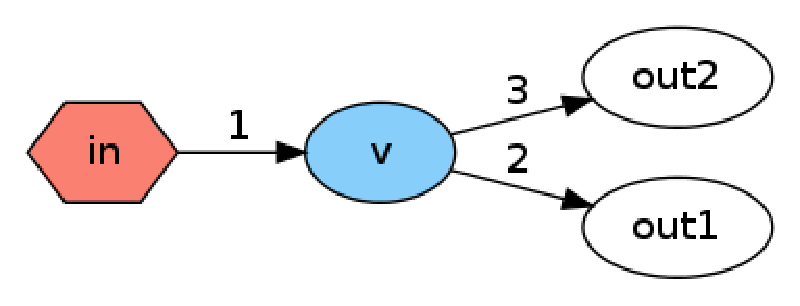
\includegraphics[width=80mm]{nadrazi0}
  \caption{Vizualizace nádraží č. 1}
  \label{fig:nad1}
\end{figure}


\subsubsection{Výhybky} výhybky jsou řízeny vzhledem k přítomnosti vlaku v nádraží a jeho cíle.
Výhybka se sepne do polohy dle cesty v grafu.
\begin{equation}
\begin{split}
\forall t,z,y:&\;
(( 
diverge(z) 
\wedge edge(z,y) \wedge\\
\wedge &\; \exists x,u: (output(u) 
						\wedge at(t,x,u) \wedge \\
						\wedge &\; (path(x,z) \vee (x = z)) \wedge \\
						\wedge &\; (path(y,u) \vee (y = u))   )) \Rightarrow \\ 
						\Rightarrow &\; branch(t,z,y)  )\\
\end{split}
\end{equation}


\begin{figure}[!h] %
  \centering
  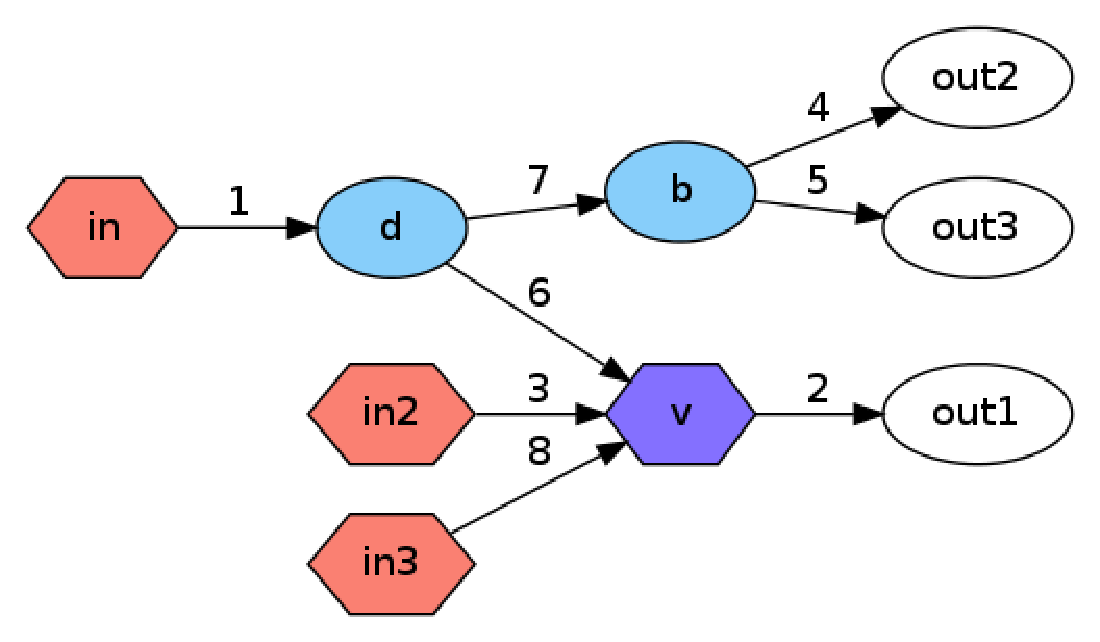
\includegraphics[width=80mm]{nadrazi1}
  \caption{Vizualizace nádraží č. 2}
  \label{fig:nad2}
\end{figure}

\subsection{Domněnky}
Dle zadánní je možné formulovat nasledujíci domněnky, které je mozno testovat vůči výše uveděné formalizaci:
\begin{itemize}
\item v nádraží nikdy nenastane kritický stav,
\item vlaky nejsou na vstupu zadržvány a jsou pouštěny jakmile je to možné.
\end{itemize}

První domněnku by bylo možné formulovat následovne:

\begin{equation}\label{eq:crit}
\begin{split}
\forall t:&\;(\forall x,u:(at(t,x,u) \wedge input(x) \wedge output(u)) \Rightarrow\\
\Rightarrow &\;\neg \exists t_1:(less(t,t_1) \wedge crit(t_1)))\\
\end{split}
\end{equation}
t.j. pro kazdy možný výskyt vlaku na vstupu, směuřujícího do výstupu platí, že neexistuje časový 
okamžik v budoucnosti, kde by nastal kritický stav.

Další domněnka říká, že je-li na vstupu i výstupu vlak tak v dalsim časovém okamžiku se nádraží uvolní
a čekající vlak se vpustí:
\begin{equation}\label{eq:crit}
\begin{split}
\forall t,x: (input(x) \wedge(\exists&\; u,v:\\
output(u) &\;\wedge output(v) \wedge\\
\wedge  at(t,x,u) &\;\wedge at(t,v,v) )) \Rightarrow \\
&\;\Rightarrow signal(succ(t),x)\\
\end{split}
\end{equation}


\begin{figure}[!h] %
  \centering
  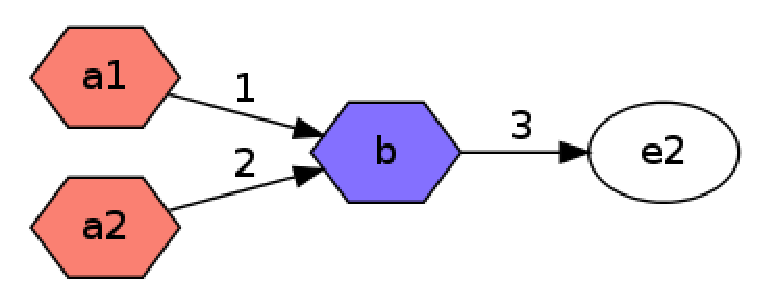
\includegraphics[width=80mm]{nadrazi2}
  \caption{Vizualizace nádraží č. 3}
  \label{fig:nad3}
\end{figure}
\section{Implementace}\label{sec:imple}
V této sekci následuje popis prostředí pro automatizovanou vefifikaci popsaného problému.

Vstupem pro tento systém je jednoduchý popis nádraží ve formátu DOT \cite{Graphviz} a výstupem 
jsou logické formule ve formátu TPTP\cite{TPTP}.

Systém byl vytvořen v jazyku \textbf{Python 2.7.3} \cite{Python}. Dále je použitý nástroj \textbf{GNU Make 3.81} \cite{GNUMake},
ktorý ulehčuje tvormu skriptů. Je to potřebné kvůli automatickému spouštení různých programů, které dohromady tvoří popisovaný systém.

Pro účely této práce byl vytvořen jazyku Python modul \textbf{pytptp}.
Je určen k manipulaci s derivačním stromem logických formulí.
Formule a její elementy jsou reprezentovány objekty, pričem je použito přetížení aritmetických a logických operací 
a tím dochází k zjednodušení zápisu výrazů logiky prvního řádu v jazyce Python.
Formule může být exportována do formátu TPTP, případně \LaTeX.
Formát TPTP pak lze použít jako vstup pro automatické dokazovače.




\subsection{Instalace a ovládání}
Po rozbalení balíku \url{http://pborky.sk/download/au.tar.gz} je kořenovém adresáři program \texttt{generator.py} a další podpůrné soubory.  
Po spuštění příkazu
\begin{verbatim}
python generator.py tpt < in/nadrazi0.in
\end{verbatim}
případne
\begin{verbatim}
make a FILE="in/nadrazi0.in"
\end{verbatim}
dojde ke zpracování souboru \texttt{nadrazi0.in} a k zobrazení logických formulí na standartní výstup. 

Zároveň budou v aktualním adresári vytvořeny
soubory \texttt{ltl.tpt} (obsahuje axiomy LTL), \texttt{control.tpt} (obsahuje axiomy pro řídící systém), 
\texttt{graph.tpt}	(axiomy nádraží, pohybu vlaku a kritických stavů), 
\texttt{t0.tpt} (test ,,vůle'' strojvůdce), \texttt{t1.tpt} (test, že se vlak vždy dostane ze vstupu na požadovaný výstup), 
\texttt{t2.tpt} (test, že nenastane kritický stav) a \texttt{t3.tpt} (test  signalizace - musí pouštět vlk jakmile to je možné).
Pomocí direktivy include jsou v adresáři \texttt{tests/} pripraveny testy, pro úkoly dle zadání:
\begin{itemize}
\item důkaz, že formalizace ,,fyzikálního chování'' nádraží není sporná,
\item důkaz, že formalizace nádraží a jeho řízení není sporná,
\item důkaz, že nikdy nenastane kritický stav,
\item a důkaz, že nádraží pouští vlaky jakmile je to možné.
\end{itemize}

Po správném nastavení cesty k programům \textbf{Prover9} alebo \textbf{Mace4} v souboru \texttt{Makefile} je možno spustit testy s dokazovači \textbf{Mace4} a \textbf{Prover9} pomocí příkazu
\begin{verbatim}
make verify
\end{verbatim}
případně
\begin{verbatim}
make verify FILE="in/nadrazi0.in"
\end{verbatim}
Vynecháním promenné \texttt{FILE} dojde ke zpracování všech soubor~u v adresáři \texttt{in/}. Do adresáře \texttt{out/}
se uloží soubory ve formátu TPT a v adresáři \texttt{logs/} budou výstupy programů \textbf{Mace4} a \textbf{Prover9}.



\section{Experimenty a závěr} \label{sec:exp}
Formalizace řešených problémů je v sekci \ref{sec:formal}. Formalizováno bylo jak ,,fyzikální`` chování nádraží 
tak aj jeho řízení. V této sekci se zaměřuje na automativké ověření správnosti zmíněné formalizace.
Za tímto účelem byl vytvořen softvér, ktorého stručný popis je v sekci \ref{sec:imple}.

Instance na, kterých byli experimenty prevedeny jsou na obr. \ref{fig:nad1}, \ref{fig:nad2} a \ref{fig:nad3}.

Experimenty byly provedeny s automatickými dokazovači \textbf{E}\cite{Eprover}, \textbf{Vampire}\cite{Vprover} 
, \textbf{Prover9} \cite{prover9-mace4} a hledadačem modelů \textbf{Mace4} \cite{prover9-mace4}.

Přiloženy jsou výsledky pouze z dokazovače \textbf{Prover9} a \textbf{Mace4} a jsou přístupné v adresáři \texttt{logs/}. 
Úkoly, kde je potřebné dokázat, že axiomy nejsou sporné, byly testovány pomocí \textbf{Mace4}.

V adresáři \texttt{tests/} jsou soubory \texttt{run1.tpt.mace4}, \texttt{run2.tpt.mace4},
\texttt{run5.tpt.prover9} a \texttt{run6.tpt.prover9}, které obsahují jenom direktivy
\texttt{include} jazyka TPT. 

Test \textbf{run1} je vytvořen pro ověření konzistence modelu nádraží a test
\textbf{run2} zahrňuje i axiomy řízení. Oba jsou předány k spracování programu \textbf{Mace4}.
Z teorie byl vypušten axiom (\ref{eq:succ_neq}) kvůli urychlení zpracování. 
Test \textbf{run1} byl proveden poměrně snadno -- viď. výstupy \texttt{nadrazi?\_run1.log}.
Problematické ale bylo hledání modelu po přidání axiomů řízení (t.j. \textbf{run2}). Problém byl způsobený axiomama (\ref{eq:flop}) a
(\ref{eq:flop1}) resp. (\ref{eq:flop2}). Z nich je možno odvodit původně vyloučený axiom (\ref{eq:succ_neq}). 
Právě proto byl vypuštěn i axiom (\ref{eq:flop}). 

Pro řešení dalších stanovených úkolů -- t.j. důkaz, že nikdy nenastane kritický stav a dále okamžité pouštění vlaku do nádraží -- 
jsou určeny testy \textbf{run5} a \textbf{run6}. Test \textbf{run6} nebylo možné verifikovat v přednastaveném čase 120sec. 
Důkaz správnosti \textbf{run5}, t.j. že v nádraží nenastane kritický stav. je v přiloženém souboru \texttt{nadrazi?\_run5.log}.



\bibliographystyle{plain}	% (uses file "plain.bst")
\bibliography{references}	
%
%\onecolumn
%\clearpage
%\appendix

%Export axiomů do formátu \LaTeX. Export byl sputěn pro nádraží
%\texttt{digraph nadrazi \{ in -> v ; v -> out1; v -> out2; \}}.
%
%\paragraph{Axiomy LTL a definice přímého následníka}
%\begin{equation*}
%\begin{split}
%\forall X,Y:(((less(X,Y) \wedge less(Y,X)) \Rightarrow (X = Y)))
%\end{split}
%\end{equation*}
%
%
%\begin{equation*}
%\begin{split}
%\forall X,Y,Z:(((less(X,Y) \wedge less(Y,Z)) \Rightarrow less(X,Z)))
%\end{split}
%\end{equation*}
%
%
%\begin{equation*}
%\begin{split}
%\forall X,Y:((less(X,Y) \vee less(Y,X)))
%\end{split}
%\end{equation*}
%
%
%\begin{equation*}
%\begin{split}
%\forall X:((less(X,succ(X)) \wedge \forall Y:((less(Y,X) \vee less(succ(X),Y)))))
%\end{split}
%\end{equation*}
%
%
%\begin{equation*}
%\begin{split}
%\forall X:((succ(X) \neq X))
%\end{split}
%\end{equation*}
%
%\paragraph{Axiomy grafu}
%\begin{equation*}
%\begin{split}
%(&\neg edge(out1,out1) \wedge \neg edge(out1,out2) \wedge \neg edge(out1,in)\wedge\\
% &\wedge \neg edge(out1,v) \wedge \neg edge(out2,out1) \wedge \neg edge(out2,out2) \wedge\\
% &\wedge \neg edge(out2,in) \wedge \neg edge(out2,v) \wedge \neg edge(in,out1) \wedge \neg edge(in,out2) \wedge\\
% &\wedge \neg edge(in,in) \wedge edge(in,v) \wedge edge(v,out1) \wedge edge(v,out2) \wedge \\
% &\wedge\neg edge(v,in) \wedge \neg edge(v,v))\\
%\end{split}
%\end{equation*}
%
%
%
%\begin{equation*}
%\begin{split}
%\forall X,Y,Z:(((path(X,Z) \wedge path(Z,Y)) \Rightarrow path(X,Y)))
%\end{split}
%\end{equation*}
%
%
%\begin{equation*}
%\begin{split}
%\forall X,Y:((edge(X,Y) \Rightarrow path(X,Y)))
%\end{split}
%\end{equation*}
%
%
%
%\begin{equation*}
%\begin{split}
%\forall X:((input(X) \Leftrightarrow (X = in)))
%\end{split}
%\end{equation*}
%
%
%\begin{equation*}
%\begin{split}
%\forall X:((output(X) \Leftrightarrow ((X = out1) \vee (X = out2))))
%\end{split}
%\end{equation*}
%
%
%\begin{equation*}
%\begin{split}
%\forall X:((diverge(X) \Leftrightarrow (X = v)))
%\end{split}
%\end{equation*}
%
%
%
%\paragraph{Axiom pohybu vlaku}
%\begin{equation*}
%\begin{split}
%&\forall T,Y,U:((at(succ(T),Y,U) \Leftrightarrow ((at(T,Y,U) \wedge (\neg want(T,Y) \vee (input(Y) \wedge \neg signal(T,Y)))) \vee\\
%&\vee \exists X:((edge(X,Y) \wedge at(T,X,U) \wedge want(T,X) \wedge ((input(X) \wedge signal(T,X)) \vee (diverge(X) \wedge branch(T,X,Y)) \vee\\
%&\vee (\neg input(X) \wedge \neg diverge(X))))))))
%\end{split}
%\end{equation*}
%
%
%
%
%\paragraph{Axiom kolize vlaků}
%\begin{equation*}
%\begin{split}
%&\forall T:((\exists X,Y:((at(T,X,U) \wedge (\neg want(T,X) \vee (input(Y) \wedge \neg signal(T,Y))) \wedge\\
%&\wedge \exists Y,V:((at(T,Y,V) \wedge edge(Y,X) \wedge want(T,Y) \wedge ((input(Y) \wedge signal(T,Y)) \vee\\
%&\vee (diverge(Y) \wedge branch(T,Y,X)) \vee (\neg input(Y) \wedge \neg diverge(Y))))))) \Rightarrow\\
%&\Rightarrow crit(succ(T))))
%\end{split}
%\end{equation*}
%
%
%\paragraph{Axiom kolize ve výhybce}
%\begin{equation*}
%\begin{split}
%&\forall T:((\exists X,U:((diverge(X) \wedge at(T,X,U) \wedge \exists Y,Z:(((Z \neq Y) \wedge branch(T,X,Y) \wedge branch(succ(T),X,Z))))) \Rightarrow\\
%&\Rightarrow crit(succ(T))))
%\end{split}
%\end{equation*}
%
%
%\paragraph{Axiom uvíznutí na vstupu}
%\begin{equation*}
%\begin{split}
%\forall T:((\exists X,U:((input(X) \wedge at(T,X,U) \wedge \neg \exists T1:((less(T,T1) \wedge signal(T1,X))))) \Rightarrow crit(T)))
%\end{split}
%\end{equation*}
%
%\paragraph{Axiom vůle strojvedoucího}
%\begin{equation*}
%\begin{split}
%\forall T,X,U:((at(T,X,U) \Rightarrow \exists T1:((less(T,T1) \wedge \forall T2:((less(T1,T2) \wedge want(T1,X)))))))
%\end{split}
%\end{equation*}
%
%
%\paragraph{Axiom blokace vstupu jedoucím vlakem}
%\begin{equation*}
%\begin{split}
%&\forall T,Z:(((input(Z) \wedge \exists X:((\exists U:(at(T,X,U)) \wedge \neg input(X) \wedge (Z \neq X) \wedge \neg \exists Y:((path(X,Y) \wedge path(Y,Z)))))) \Rightarrow\\
%&\Rightarrow block(T,Z)))
%\end{split}
%\end{equation*}
%
%
%\paragraph{Axiom časovače řízení vstupního semaforu (u jednoho vstupu je trvale sepnutý)}
%\begin{equation*}
%\begin{split}
%\forall T:(flop(T,in))
%\end{split}
%\end{equation*}
%
%
%\paragraph{Axiom řízení vstupního semaforu}
%\begin{equation*}
%\begin{split}
%(\forall T,X:((input(X) \wedge flop(T,X) \wedge \neg block(T,X))) \Rightarrow signal(T,X))
%\end{split}
%\end{equation*}
%
%
%\paragraph{Axiom řízení výhybky}
%\begin{equation*}
%\begin{split}
%&\forall T,Z,Y:(((diverge(Z) \wedge edge(Z,Y) \wedge \exists X,U:((at(T,X,U) \wedge (path(X,Z) \vee (X = Z)) \wedge (path(Y,U) \vee (Y = U))))) \Rightarrow\\
%&\Rightarrow branch(T,Z,Y)))
%\end{split}
%\end{equation*}
%
%
%\paragraph{Axiom okamžitého vypuštení vlaku}
%\begin{equation*}
%\begin{split}
%\forall T,X,U:((at(T,X,U) \Rightarrow want(T,X)))
%\end{split}
%\end{equation*}
%
%
%\paragraph{Test uváznutí na vstupu}
%\begin{equation*}
%\begin{split}
%&\forall T,X,U:(((input(X) \wedge output(U) \wedge at(T,X,U) \wedge \neg \exists Y:((\neg input(Y) \wedge \exists V:(at(T,Y,V))))) \Rightarrow\\
%&\Rightarrow \exists T1:((less(T,T1) \wedge (T \neq T1) \wedge at(T1,U,U)))))
%\end{split}
%\end{equation*}
%
%
%\paragraph{Test výskytu kritického stavu}
%\begin{equation*}
%\begin{split}
%\forall T:((\forall X,U:((at(T,X,U) \wedge input(X) \wedge output(U))) \Rightarrow \neg \exists T1:((less(T,T1) \wedge crit(T1)))))
%\end{split}
%\end{equation*}
%
%
%\paragraph{Test okamžitého vypuštení vlaku}
%\begin{equation*}
%\begin{split}
%\forall T:(\exists X:((\exists U,V:((at(T,X,U) \wedge input(X) \wedge output(U) \wedge at(T,V,U) \wedge output(V) \wedge block(T,X) \wedge\\ \neg \exists Y,Z:((\neg input(Y) \wedge \neg output(Y) \wedge at(T,Y,Z))))) \Rightarrow signal(T,X))))\\
%\end{split}
%\end{equation*}





% that's all folks
\end{document}
